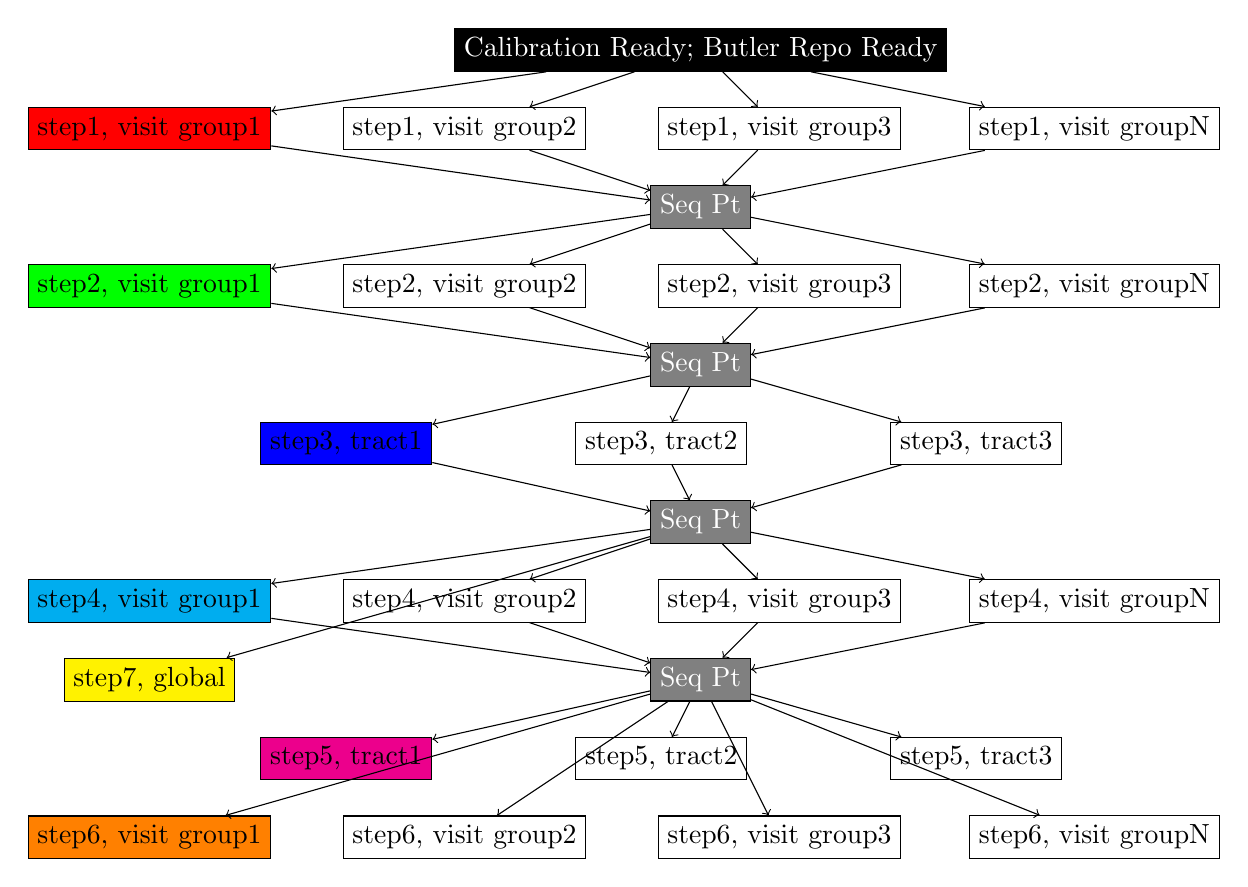
\begin{tikzpicture}[->]
  \node[draw,fill=black,text=white] (step0) at (10,10) {Calibration Ready; Butler Repo Ready};

  \node[draw,fill=red] (step1v1) at (3,9) {step1, visit group1};
  \node[draw] (step1v2) at (7,9) {step1, visit group2};
  \node[draw] (step1v3) at (11,9) {step1, visit group3};
  \node[draw] (step1v4) at (15,9) {step1, visit groupN};
  \foreach \to in {step1v1,step1v2,step1v3,step1v4}
    \draw (step0) -- (\to);

  \node[draw,fill=gray,text=white] (sq1) at (10,8) {Seq Pt};
  \foreach \from in {step1v1,step1v2,step1v3,step1v4}
    \draw (\from) -- (sq1);

  \node[draw,fill=green] (step2v1) at (3,7) {step2, visit group1};
  \node[draw] (step2v2) at (7,7) {step2, visit group2};
  \node[draw] (step2v3) at (11,7) {step2, visit group3};
  \node[draw] (step2v4) at (15,7) {step2, visit groupN};
  \foreach \to in {step2v1,step2v2,step2v3,step2v4}
    \draw (sq1) -- (\to);

  \node[draw,fill=gray,text=white] (sq2) at (10,6) {Seq Pt};
  \foreach \from in {step2v1,step2v2,step2v3,step2v4}
    \draw (\from) -- (sq2);

  \node[draw,fill=blue] (step3v1) at (5.5,5) {step3, tract1};
  \node[draw] (step3v2) at (9.5,5) {step3, tract2};
  \node[draw] (step3v3) at (13.5,5) {step3, tract3};
  \foreach \to in {step3v1,step3v2,step3v3}
    \draw (sq2) -- (\to);

  \node[draw,fill=gray,text=white] (sq3) at (10,4) {Seq Pt};
  \foreach \from in {step3v1,step3v2,step3v3}
    \draw (\from) -- (sq3);

  \node[draw,fill=cyan] (step4v1) at (3,3) {step4, visit group1};
  \node[draw] (step4v2) at (7,3) {step4, visit group2};
  \node[draw] (step4v3) at (11,3) {step4, visit group3};
  \node[draw] (step4v4) at (15,3) {step4, visit groupN};
  \foreach \to in {step4v1,step4v2,step4v3,step4v4}
    \draw (sq3) -- (\to);

  \node[draw,fill=gray,text=white] (sq4) at (10,2) {Seq Pt};
  \foreach \from in {step4v1,step4v2,step4v3,step4v4}
    \draw (\from) -- (sq4);

  \node[draw,fill=yellow] (step7) at (3, 2) {step7, global};
  \draw (sq3) -- (step7);

  \node[draw,fill=magenta] (step5v1) at (5.5,1) {step5, tract1};
  \node[draw] (step5v2) at (9.5,1) {step5, tract2};
  \node[draw] (step5v3) at (13.5,1) {step5, tract3};
  \foreach \to in {step5v1,step5v2,step5v3}
    \draw (sq4) -- (\to);

  %\node[draw,fill=gray,text=white] (sq4) at (10,0) {Seq Pt};
  %\foreach \from in {step4v1,step4v2,step4v3,step4v4}
  %  \draw (\from) -- (sq4);

  \node[draw,fill=orange] (step6v1) at (3,0) {step6, visit group1};
  \node[draw] (step6v2) at (7,0) {step6, visit group2};
  \node[draw] (step6v3) at (11,0) {step6, visit group3};
  \node[draw] (step6v4) at (15,0) {step6, visit groupN};
  \foreach \to in {step6v1,step6v2,step6v3,step6v4}
    \draw (sq4) -- (\to);

\end{tikzpicture}
